\documentclass[a4paper]{article}
\usepackage[a4paper,left=3cm,right=2cm,top=2.5cm,bottom=2.5cm]{geometry}
\usepackage[utf8]{inputenc}
\usepackage{amsmath}
\usepackage{graphicx}
\graphicspath{ {./images/} }

\title{\textbf{Intel·ligència Artificial:\\
Pràctica de Cerca Local}}
\author{\emph{Pol Marcet, Pablo Vega, Adrià Fernández}}
\date{Curs 2021-2022, Semestre de Tardor}

\renewcommand*\contentsname{Continguts}
\renewcommand{\figurename}{Figura}

\begin{document}

\begin{titlepage}
\clearpage\maketitle
\thispagestyle{empty}
\end{titlepage}

\tableofcontents
\clearpage

\section{Part Descriptiva}

\subsection{Descripció del Problema}
El problema ens planteja una companyia de distribució de combustible que vol abastir una sèrie de gasolineres, maximitzant el seu benefici. En un taulell de 100x100 quilòmetres hi ha distribuïts \emph{n} centres de distribució i \emph{g} gasolineres. La distancia entre dos elements A i B es calcula seguint la següent fórmula:

\begin{center}
$d(A,B) = |A_x-B_x|+|A_y-B_y|$
\end{center}

Les gasolineres disposen d'una sèrie de dipòsits. Quan un dipòsit es buida completament la gasolinera emet una petició, que un centre de distribució haurà de complir. Les peticions que romanen sense atendre al final del dia s'assumeix que són ateses l'endemà. El valor del dipòsit pateix una depreciació segons el nombre de dies que no ha estat atesa, seguint la següent fórmula:

\[
\%preu = \left\{\begin{array}{lr}
102\%, & \text{si } dies = 0\\
(100-2^{dies})\%, & \text{si } dies > 0\\
\end{array}\right\}
\]\

Cada centre de distribució disposa d'un camió amb capacitat equivalent a dos dipòsits. Un camió realitza una sèrie de viatges per atendre peticions. Després d'atendre com a molt dues peticions (que poden ser de la mateixa gasolinera), el camió haurà de tornar al seu centre de distribució per reomplir-se. Tant el nombre de viatges que pot realitzar com els quilòmetres totals que pot recórrer un camió estan limitats. Cada quilòmetre que recorre un camió té un cost fix, i per tant per maximitzar els beneficis ens interessa minimitzar el recorregut.\\

Per realitzar el problema, i facilitar les experimentacions, hem definit les següents variables globals:
\begin{itemize}
\item Nombre de gasolineres. Per defecte 100.
\item Nombre de centres de distribució. Per defecte 10.
\item Superposició de centres de distribució, que permet simular més d'un camió per centre. Per defecte 1.
\item Preu per quilòmetre que recorre el camió. Per defecte 2.
\item Màxim de quilòmetres que pot recorre un camió. Per defecte 80*8.
\item Màxim de viatges que pot realitzar un camió. Per defecte 5.
\item Valor base que genera omplir un dipòsit. Per defecte 1000.
\item Llavor usada per la generació aleatòria.\\
\end{itemize}

\subsubsection{Elements del Problema}
Cada centre de distribució disposa d'un únic camió. Aquest camió sempre ha de retornar al mateix centre de distribució. Per a simular més d'un camió cal superposar diversos centres de distribució a les mateixes coordenades. És per aquests motius que hem decidit abstraure els camions de la nostra representació, i considerar-los com implícits als centres de distribució.\

Un altre element que podem ometre són les gasolineres, donat que per la resolució del problema l'únic element rellevant són les seves peticions. És a dir, no considerarem les gasolineres sense peticions, i si una gasolinera té múltiples peticions, les considerarem individualment.\\

Per tat, els elements del problema que tindrem en consideració seran els següents:
\begin{itemize}
\item \emph{Peticions}, amb les seves coordenades i dies pendents.
\item \emph{Centres de Distribució}, amb les seves coordenades, la seva ruta, els seus quilòmetres recorreguts i el seu benefici acumulat.\\
\end{itemize}

\subsubsection{Cerca Local}
Per resoldre aquest problema i trobar una ruta òptima s'utilitzarà la \emph{cerca local}, que consisteix en trobar una solució inicial i explorar els seus estats pròxims per trobar-ne un d'òptim. Aquesta metodologia té una complexitat temporal molt inferior a mètodes com el backtracking. Aquesta metodologia és una eina poderosa, donat que es compleixin les següents condicions:
\begin{itemize}
\item És un problema d'optimització pur amb l'objectiu d'obtenir el millor estat segons una funció objectiva.
\item El camí fins a arribar a un estat final és irrellevant.
\end{itemize}

És fàcil veure que es compleix la primera condició: l'objectiu del problema és maximitzar els nostres beneficis, que es poden calcular per a qualsevol estat. Però donat que cada camió realitza una sèrie de viatges durant un dia es podria assumir que el camí per arribar a la solució és important. Veiem un exemple (fig. 1):
\begin{figure}[h]
\centering
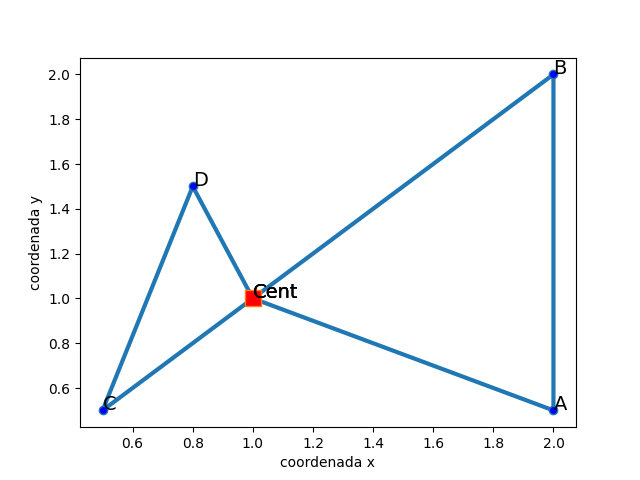
\includegraphics[scale=0.65]{images/fig1.png}
\caption{Exemple de ruta}
\centering
\end{figure}

$A, B, C, D$ representen gasolineres amb peticions, i $Cent$ representa un centre de distribució. En blau hi ha marcada la ruta del camió. Podem veure com la ruta $(Cent,A,B,Cent,D,C,Cent)$ i la ruta $(Cent,C,D,Cent,B,A,Cent)$ resultaran exactament en els mateixos beneficis, el mateix nombre de viatges i la mateixa quantitat de quilòmetres recorreguts. Per tant, podem concloure que el camí per arribar a la solució \emph{no} és important, l'únic important és l'aparellament de gasolineres.\\

Així doncs, el nostre problema compleix totes les condicions necessàries per ser resolt mitjançant la cerca local.

\subsubsection{Espai de Cerca}
L'espai de cerca es defineix com la totalitat de les solucions candidates, o estats finals, que té el nostre problema. És rellevant conèixer-lo, ja que un espai de solucions en ordre polinòmic implicaria que seria factible resoldre el nostre problema mitjançant la força bruta. També ens dona una idea de la magnitud del problema que estem afrontant.\\

Assumim que tenim $n$ centres de distribució i $m$ peticions. Considerarem el pitjor cas possible, on les distàncies són molt petites.\\

Per a un centre de distribució determinat, assumim que col·loquem les $m$ peticions en un vector de booleans, on 1 representa que atens la petició i 0 que no l'atens. Per tant l'espai de solucions estaria en l'ordre de $O(2^m)$ (o binomi de m sobre 10 si tens en compte que atens com a molt 10 peticions). Això és clarament no polinòmic i per tant no seria viable resoldre el problema per força bruta.\\

Si considerem la totalitat de centres de distribució, podem modificar el nostre vector perquè una petició tingui 0 si no és atesa, 1 si l'atén el centre de distribució 1, 2 si l'atén el centre de distribució 2,... fins a $n$ si l'atén el centre de distribució $n$. L'espai de solucions, doncs, estaria en l'ordre de $O(n^m)$.\\

Més enllà, ens caldria considerar que en cada viatge un centre de distribució pot atendre dues peticions, i doncs hem de pensar de quantes formes es poden agrupar m elements en grups de 2. Per tant l'ordre estaria en $O(\binom{m}{2} * n^m)$.\\

Amb els valors per defecte $n = 10$ i $m = 100$ tenim un espai de solucions de $4.95*10^{103}$. Per referència, s'estima que hi ha $10^{82}$ àtoms a l'univers.\\

\subsection{Implementació de l'Estat}

Una primera idea d'implementació de l'estat podria ser una matriu de 100x100 on cada cel·la representa un quilòmetre quadrat amb els seus elements. Aquesta idea va ser ràpidament descartada, ja que donat que no hi ha obstacles al tauler l'únic important és la distància entre els elements. Per tant, a la nostra representació hem decidit mantenir una matriu estàtica de les distàncies entre gasolineres (\emph{gasToGas}) i entre centres i gasolineres (\emph{distrToGas}).\\

També hem guardat de forma estàtica una matriu amb la informació de cada petició (dies pendents, coordenades) i de cada centre de distribució (coordenades), després d'assignar-los un identificador numèric.\\

Per a cada centre de distribució hem establert la classe \emph{StateDistr}. Aquesta classe emmagatzema la distància total recorreguda pel seu camió, el benefici total aconseguit pel seu camió i la ruta que prendrà el seu camió. La ruta és guardada com a una llista de gasolineres que visita. La llista té grandària com a molt 10, ja que aquest és el màxim de peticions que pot complir en un dia. Per calcular la distància hem considerat que el camió surt del centre de distribució, visita les dues primeres peticions, torna al centre de distribució i segueix així fins a arribar al final de la llista. Una implicació d'aquesta implementació és que només pot haver-hi un sol cas on el camió només atengui una sola petició abans de tornar, que serà al final. Creiem que això és positiu, donat que mai serà més eficient atendre més d'una petició individualment degut al teorema de la desigualtat del triangle.\\

Una alternativa que vam pensar va ser que cada centre de distribució tingués 5 llistes que poguessin emmagatzemar dues gasolineres. Així, aconseguiríem abstraure del tot l'ordre de visita. Vam decidir descartar aquesta opció, ja que la seva implementació més complexa no suposava una millora en el problema.\\

Finalment, hem guardat les peticions sense atendre en una llista.\\

\begin{figure}[h]
\centering
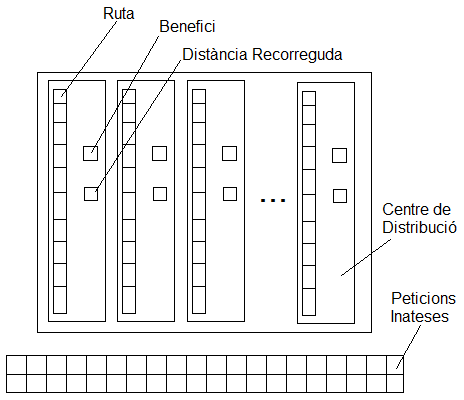
\includegraphics[scale=0.65]{images/fig2.png}
\caption{Esquema dels elements no-estàtics}
\end{figure}

Creiem que aquesta representació ens dona una forma ràpida d'afegir o eliminar peticions d'una ruta, ja que simplement les hem de moure entre les ateses i les no ateses. També creiem que ens permet comprovar les restriccions (per exemple, la distància màxima) i calcular els beneficis totals de forma eficient. En fer servir atributs estàtics minimitzem tant com podem l'espai de memòria ocupat, que serà convenient donat que l'estat es clonarà milers de vegades.\\

\newpage
\subsection{Operadors del Problema}
Per modificar l'estat hem implementat els següents operadors. Pel càlcul del factor de ramificació assumim que tenim $n$ centres de distribució i $m$ peticions.

\paragraph{Afegir}
\begin{itemize}
\item \emph{Paràmetres:} l'índex d'un centre de distribució $i$, l'índex d'una petició sense atendre $j$, un nombre enter $k$.
\item \emph{Precondicions:} el centre de distribució $i$ atén a menys de 10 peticions, entre les quals no es troba la petició $j$. L'enter $k$ és menor o igual que 10.
\item \emph{Postcondicions:} S'afegeix la petició $j$ a la ruta del centre $i$ en la posició $k$. La petició $j$ és esborrada de les peticions sense atendre. S'actualitzen els beneficis i la distància, que ha de ser menor o igual que el màxim permès.
\item \emph{Factor de Ramificació:} Qualsevol petició pot anar a qualsevol centre de distribució en qualsevol de les 10 posicions, per tant, és a l'ordre de $O(n*m*10)$.
\end{itemize}

\paragraph{Eliminar}
\begin{itemize}
\item \emph{Paràmetres:} l'índex d'un centre de distribució $i$, l'índex d'una petició $j$.
\item \emph{Precondicions:} el centre de distribució $i$ atén la petició $j$.
\item \emph{Postcondicions:} el centre de distribució $i$ deixa d'atendre la petició $j$. La petició $j$ es afegida a les peticions sense atendre. Es recalculen les distàncies i els beneficis.
\item \emph{Factor de Ramificació:} Es pot eliminar una de les 10 peticions de qualsevol centre de distribució. Per tant, és a l'ordre de $O(n*10)$.
\end{itemize}

\paragraph{Rotar}
\begin{itemize}
\item \emph{Paràmetres:} l'índex d'un centre de distribució $i$.
\item \emph{Precondicions:} -.
\item \emph{Postcondicions:} la ruta del centre de distribució $i$ rota una posició. És a dir, el primer element passa a ser l'últim i es refan les parelles. Es recalcula la distància i els beneficis, que no pot superar els quilòmetres màxims.
\item \emph{Factor de Ramificació:} Es pot rotar qualsevol centre de distribució, per tant, és a l'ordre de $O(n)$.
\end{itemize}

\paragraph{Moure}
\begin{itemize}
\item \emph{Paràmetres:} l'índex d'un centre de distribució $i$, l'índex d'un centre de distribució $j$, l'índex d'una petició $ip$, un enter $k$.
\item \emph{Precondicions:} els centres de distribució $i$ i $j$ són diferents. El centre de distribució $i$ atén la petició $ip$. El centre de distribució $j$ no l'atén. L'enter $k$ és menor o igual que 10.
\item \emph{Postcondicions:} la petició $ip$ deixa de ser atesa per $i$ i passa a ser atesa per $j$ en l'índex $k$. Es recalculen els beneficis i les distàncies, que no poden superar el màxim.
\item \emph{Factor de Ramificació:} Es pot moure la petició de qualsevol centre de distribució a qualsevol altre centre. Donat que cada ruta té 10 posicions el factor de ramificació és de $O(n^2*10^2)$.
\end{itemize}

\paragraph{Intercanviar (Propi)}
\begin{itemize}
\item \emph{Paràmetres:} l'índex d'un centre de distribució $i$. Dos enters $k1$ i $k2$.
\item \emph{Precondicions:} -.
\item \emph{Postcondicions:} la petició situada a la posició $k1$ del centre de distribució $i$ passa a estar a la posició $k2$. Es recalculen els beneficis i la distància, que no pot superar el màxim.
\item \emph{Factor de Ramificació:} es pot operar sobre qualsevol centre de distribució, i intercanviar dos índexs qualssevol, Per tant, és a l'ordre de $O(n*10^2)$.
\end{itemize}

\paragraph{Intercanviar (Altre)}
\begin{itemize}
\item \emph{Paràmetres:} l'índex d'un centre de distribució $i$, l'índex d'un centre de distribució $j$, l'índex d'una petició $ip$, l'índex d'una petició $jp$.
\item \emph{Precondicions:} els centres de distribució $i$ i $j$ són diferents. El centre de distribució $i$ aten la petició $ip$ i no atén a la petició $jp$, i viceversa.
\item \emph{Postcondicions:} la petició $ip$ i la petició $jp$ intercanvien centre de distribució i posició. Es recalculen beneficis i distancies, que no poden superar el màxim.
\item \emph{Factor de Ramificació:} Es pot moure la petició de qualsevol centre de distribució a qualsevol altre centre. Donat que cada ruta té 10 posicions el factor de ramificació és de $O(n^2*10^2)$.
\end{itemize}

\paragraph{Intercanviar (Doble)}
\begin{itemize}
\item \emph{Paràmetres:} l'índex d'un centre de distribució $i$, l'índex d'un centre de distribució $j$, l'índex d'una petició $ip$, l'índex d'una petició $jp$.
\item \emph{Precondicions:} els centres de distribució $i$ i $j$ són diferents. El centre de distribució $i$ aten la petició $ip$ i no atén a la petició $jp$, i viceversa. Els índexs $ip$ i $jp$ són parells i no corresponen a l'última petició del centre.
\item \emph{Postcondicions:} les peticions $(ip, ip+1)$ i les peticions $(jp, jp+1)$ intercanvien centres de distribució i posicións. Es recalculen beneficis i distancies, que no poden superar el màxim.
\item \emph{Factor de Ramificació:} Es pot moure la petició de qualsevol centre de distribució a qualsevol altre centre. Donat que cada ruta té 10 posicions el factor de ramificació és de $O(n^2*10^2)$.\\
\end{itemize}

Creiem que aquests operadors poden tots suposar millores de l'estat, i que exploren un espai de solucions molt ampli conjuntament. A la part experimental hem comprovat que això és cert, exceptuant l'operador Intercanviar (Doble) i l'operador Moure, que finalment hem eliminat. Tenim un nombre elevat d'operadors en comparació amb els exemples vistos a classe, però creiem que això és positiu ja que ens permet explorar gran quantitat d'estats possibles. Els nostres operadors tenen un comportament generalitzable a altres problemes, i ens serà útil en futurs problemes.\\

\subsection{Generació de Solucions Inicials}
Per la realització del treball hem implementat tres mètodes diferents de generació d'estat inicial:

\paragraph{Buit}
Aquest estat inicial consisteix en el taulell completament buit, sense que cap centre de distribució atengui cap petició. Generar aquesta solució inicial és computacionalment negligible. Comença amb benefici zero. Creiem que té la avantatja que en començar en buit l'algorisme de Hill Climbing resoldrà el problema de forma semblant a un algorisme voraç, fent servir gairebé exclusivament els operadors d'afegir.

\begin{figure}[th]
\centering
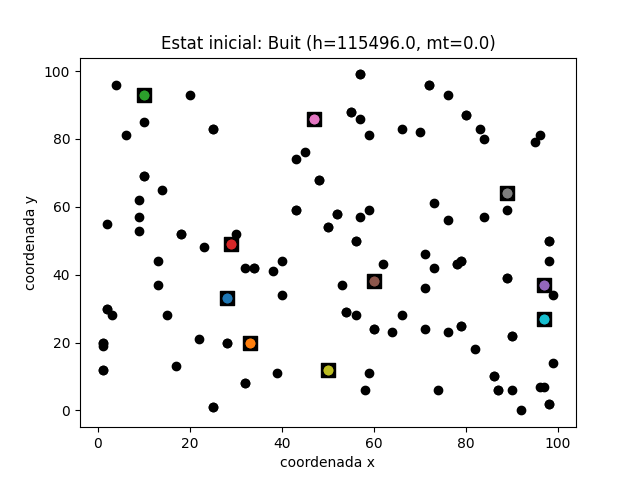
\includegraphics[scale=0.6]{images/fig3.png}
\caption{Exemple d'estat inicial Buit}
\end{figure}

\paragraph{Més Proper}
En aquest estat inicial cada centre de distribució atén a la petició més propera. Generar aquesta solució consisteix en, per a cada centre, recórrer linealment les distàncies entre centres i gasolineres i afegir la més propera. La seva bondat és lleugerament millor que la Buida completament. Creiem que aquesta generació inicial té valor, ja que encamina la solució cap a un camí raonable.

\begin{figure}[th]
\centering
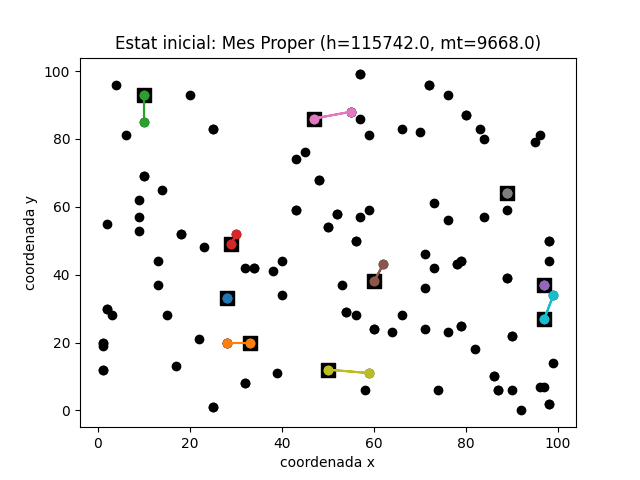
\includegraphics[scale=0.6]{images/fig4.png}
\caption{Exemple d'estat inicial Més Proper}
\end{figure}

\paragraph{Tants Possibles}
Aquest estat inicial consisteix a iterar en bucle sobre els centres de distribució, i a cada pas afegir-hi la gasolinera més propera si ho permet la distància, fins que totes siguin plenes o no quedin més peticions. El seu cost computacional és bastant elevat, ja que recorre linealment les distàncies per a cada centre a cada iteració del bucle (tot i que es podria reduir considerablement implementant una cua de prioritats). A canvi, però, aquest estat inicial genera una solució amb molt bona bondat, i per tant caldran pocs passos fins que l'heurística arribi a una vall.

\begin{figure}[th]
\centering
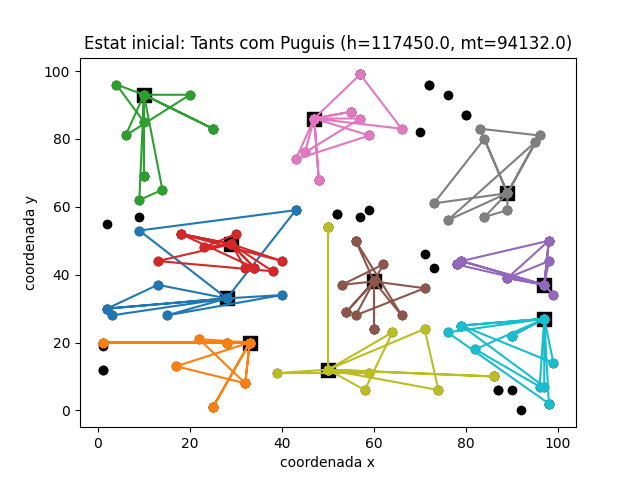
\includegraphics[scale=0.6]{images/fig5.png}
\caption{Exemple d'estat inicial Tants Possibles}
\end{figure}

\subsection{Funció Heurística}
La nostra funció heurística calcula, per a cada centre de distribució, el total de beneficis que genera omplint dipòsit i els resta el cost dels quilòmetres recorreguts.\\

Donat que s'assumeix que l'endemà s'atenen les peticions que romanen sense atendre també sumem el benefici que suposaries atendre-les l'endemà. A les peticions sense atendre els hem restat cost de viatjar-hi des del centre de distribució més proper, ja que altrament es podria donar la situació que prioritzés no atendre una petició a atendre-la. Una altre forma de tractar les peticions sense atendre plantejada era restar a la heurística les pèrdues que suposaria tractar la petició a l'endema respecte tractar-les avui.\\

Una altre consideració que vam realitzar va ser limitar els beneficis de complir una petició a com a mínim zero (per exemple, una petició amb 7 dies pendents donaria beneficis negatius). Finalment, vam decidir descartar aquesta opció ja que aquesta heurúistica no castiga prou deixar peticions amb molts dies pendents per l'endemà, tot i que suposaria una lleugera millora computacional en el càlcul del benefici. Adicionalment, el problema només genera peticions amb com a molt tres dies pendents.\\

Aquesta heurística és senzilla i no té ponderacions, però el seu funcionament és bó, ja que el problema posseeix una funció de bondat molt objectiva (els beneficis generats), en contrast d'altres problemes de cerca local.\\

\newpage
\subsection{Resultats}
Usant la llibreria de \emph{Matplotlib} de Python hem representat gràficament les solucions finals usant la llavor aleatòria 1234. Els quadrats representen centres de distribució i els cercels gasolineres. El valor $h$ representa l'heurística, $mt$ els diners guanyats avui i $n$ els nodes expandits. Heus aquí els resultats, emprant els valors per defecte de Simulated Annealing:

\begin{figure}[htp]
\centering
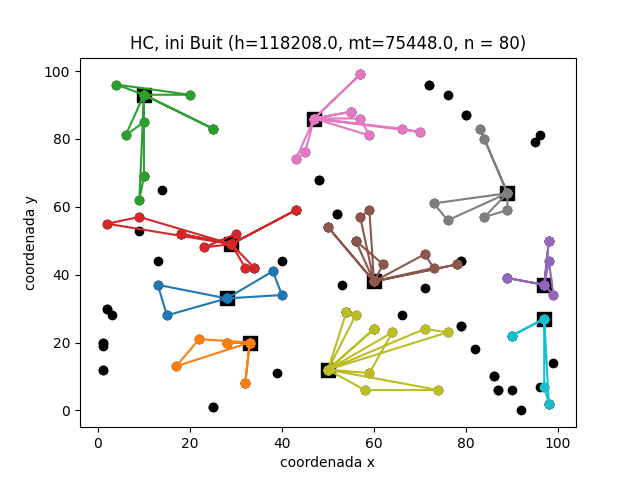
\includegraphics[scale=0.65]{images/fig6.png}
\caption{Final amb Hill Climbing, inici Buit}
\centering
\end{figure}

\begin{figure}[htp]
\centering
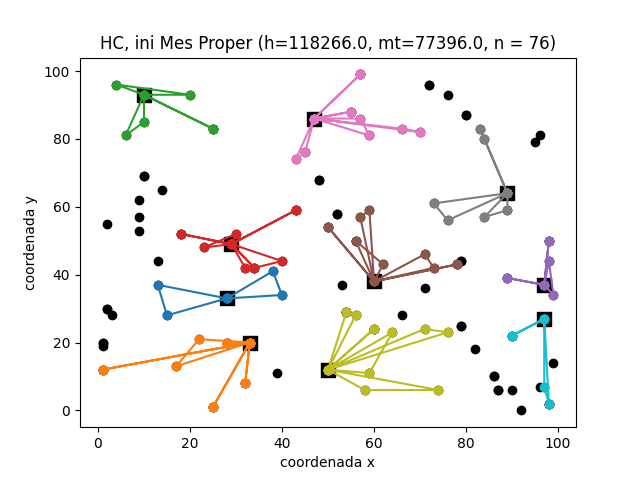
\includegraphics[scale=0.65]{images/fig7.png}
\caption{Final amb Hill Climbing, inici Més Proper}
\centering
\end{figure}

\begin{figure}[htp]
\centering
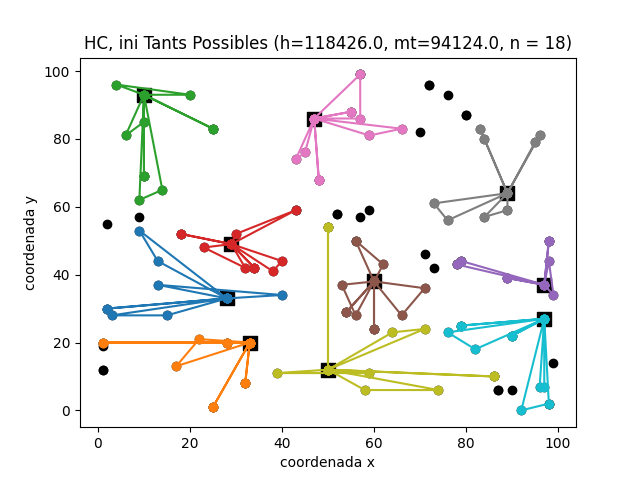
\includegraphics[scale=0.65]{images/fig8.png}
\caption{Final amb Hill Climbing, inici Tants Possibles}
\centering
\end{figure}

\begin{figure}[htp]
\centering
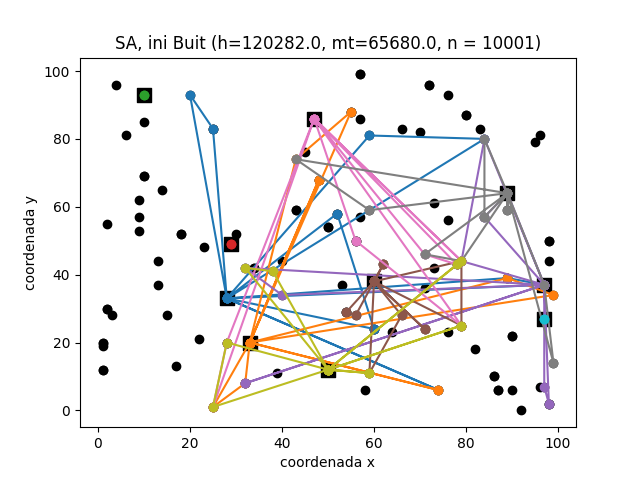
\includegraphics[scale=0.65]{images/fig9.png}
\caption{Final amb Simulated Annealing, inici Buit}
\centering
\end{figure}

\begin{figure}[htp]
\centering
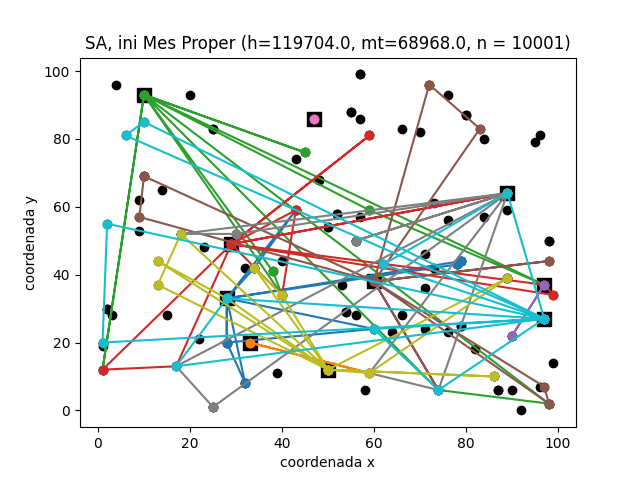
\includegraphics[scale=0.65]{images/fig10.png}
\caption{Final amb Simulated Annealing, inici Més Proper}
\centering
\end{figure}

\begin{figure}[htp]
\centering
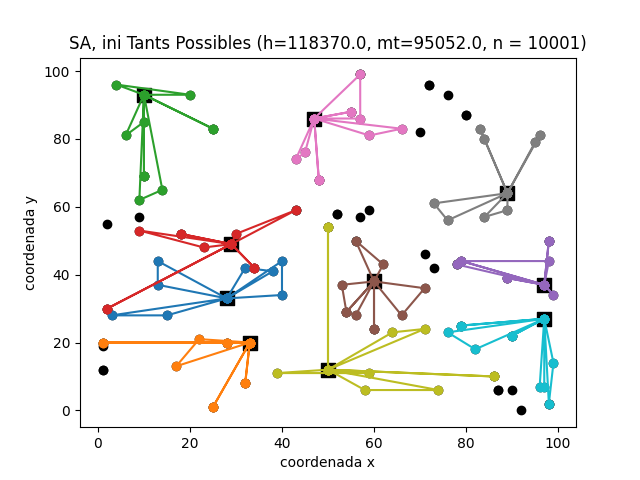
\includegraphics[scale=0.65]{images/fig11.png}
\caption{Final amb Simulated Annealing, inici Tants Possibles}
\centering
\end{figure}

\newpage
\section{Part Experimental}

\subsection{Experiment 1}
Aquest experiment ens planteja comprovar quins operadors donen el millor resultat per a poder-los fixar per la resta d'experiments. Donat que l'algorisme Hill Climbing a cada iteració fa el pas que suposa major heurística, si veiem quins operadors fa servir veurem quins operadors són útils.
\paragraph{Observació} No tots els operadors semblen ser usats per igual. Generacions inicials diferents utilitzen conjunts d'operadors molt diferents.
\paragraph{Plantejament} Quantifiquem els operadors que fa servir l'algorisme per a cada estat inicial.
\paragraph{Hipòtesi} Tant l'estat inicial Tot Buit com el Més Proper faran servir exclusivament l'operador Afegir. En canvi a l'estat inicial de Tants Possibles no hi haurà Afegirs.
\paragraph{Metodologia}
\begin{itemize}
\item Usarem els valors 10 centres de distribució i 100 gasolineres.
\item Usarem l'algorisme Hill Climbing.
\item Executarem el programa 100 vegades amb llavors de generació aleatòries.
\item Calcularem el percentatge de quants cops s'executa cada operador per a cada estat inicial.
\end{itemize}

\paragraph{Resultats} Hem obtingut els següents resultats:

\begin{figure}[htp]
\centering
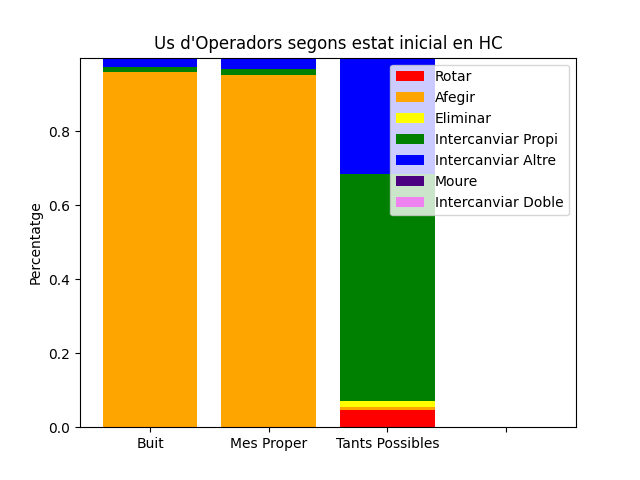
\includegraphics[scale=0.75]{images/barplots.png}
\caption{Resultats d'Inici Buit, Inici Més Proper i Inici Tants Possibles}
\centering
\end{figure}

\paragraph{Conclusions} Podem veure que les nostres hipòtesis eren bastant encertades, però els estats inicials Buit i Més Proper també fan servir, ocasionalment, altres operadors, i l'estat inicial Tants Possibles fa servir l'operador Afegir ocasionalment. Podem concloure que tots els operadors es fan servir en alguna generació d'estat inicial, amb l'excepció dels operadors Intercanviar Doble i l'operador Moure, que finalment hem decidit eliminar.

\subsection{Experiment 2}
Aquest experiment ens planteja comprovar quina generació d'estats inicials dona millor resultat.
\paragraph{Observació} No tots els estats inicials donen els mateixos resultats.
\paragraph{Plantejament} Comparem els resultats dels diferents estats inicials.
\paragraph{Hipòtesi} Hi ha dues opinions prevalents al grup: per una banda, es creu que la generació inicial Tot Buit serà la millor, ja que en ser més "golafre" prendrà la millor decisió en cada pas i per tant acabarà amb el millor resultat. Per l'altra banda, es creu que l'algorisme de generació de Tants Possibles té una heurística inicial molt bona i molt propera a una solució idònia.
\paragraph{Metodologia}
\begin{itemize}
\item Usarem els valors 10 centres de distribució i 100 gasolineres.
\item Usarem l'algorisme Hill Climbing.
\item Executarem el programa 100 vegades amb llavors de generació aleatòries per a cada estat inical.
\item Comparem els resultats de l'heurística dels diferents estats inicials.
\item Adicionalment, comparem els nodes expandits.
\end{itemize}

\paragraph{Resultats} Hem obtingut els següents resultats:

\begin{figure}[htp]
\centering
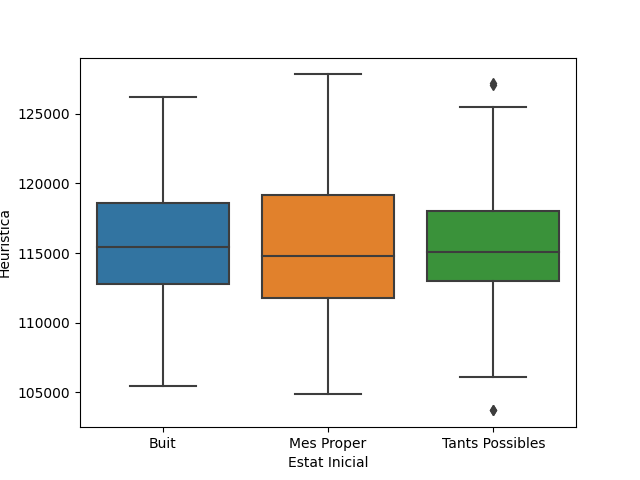
\includegraphics[scale=0.75]{images/experiment2-1.png}
\caption{Resultats de l'heurística d'Inici Buit, Inici Més Proper i Inici Tants Possibles}
\centering
\end{figure}

\begin{figure}[htp]
\centering
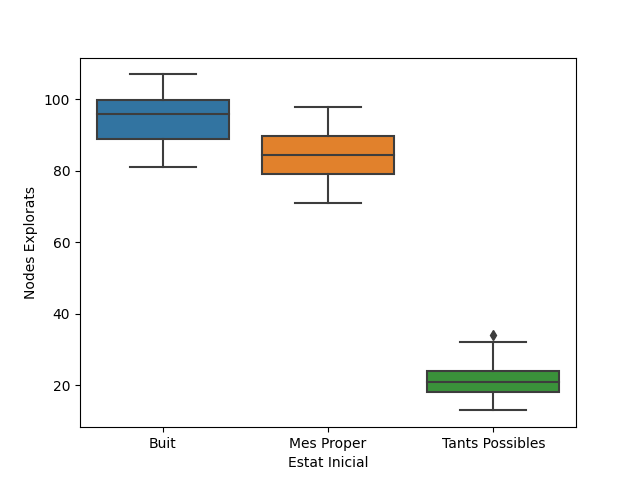
\includegraphics[scale=0.75]{images/experiment2-2.png}
\caption{Nodes Explorats per Inici Buit, Inici Més Proper i Inici Tants Possibles}
\centering
\end{figure}

\newpage
\paragraph{Conclusions} Els resultats de l'heurística són virtualment iguals, amb l'estat inicial Més Proper tenint lleugerament els millors resultats màxims. Però, si comprovem els nodes expandits de cada generació d'estat inicial, podem veure com Tants Possibles dona temps d'execució dràsticament inferiors als altres dos, a causa de la bondat de la solució inicial. Per aquest motiu hem considerat que el millor algorisme de generació d'estat inicial és Tants Possibles.\\
\newpage

\subsection{Experiment 3}
Aquest experiment ens planteja trobar els valors de $k$, $\lambda$ i $stiter$ de Simulated Annealing que generen uns millors resultats.
\paragraph{Observació} Diferents valors de Simulated Annealing generen diferents resultats.
\paragraph{Plantejament} Provem diferents valors de les variables per trobar el millor.
\paragraph{Hipòtesi} Els valors per defecte no seran els millors, però no sabríem determinar quins són els millors.
\paragraph{Metodologia}
\begin{itemize}
\item Usarem els valors 10 centres de distribució i 100 gasolineres.
\item Usarem l'algorisme Simulated Anealing, amb 10000 nombres de passos.
\item Determinem uns possibles valors de $k$, $\lambda$ i $stiter$, que seran:
\begin{itemize}
\item{$k = [1,5,25,125,625,3125]$}
\item{$\lambda = [1.0,0.1,0.01,0.001,1.0E-4,1.0E-5,1.0E-6]$}
\item{$stiter = [10,20,..,90,100]$}
\end{itemize}
\item Executarem el programa 50 vegades amb llavors de generació aleatòries per a cada combinació de variables
\item Calculem la mitjana de les 50 iteracions de cada combinació
\item Trobem la mitjana màxima entre totes les combinacions de variables
\end{itemize}

\paragraph{Resultats} Hem elaborat un gràfic dels resultats amb $stiter=100$, que conté el resultat màxim:

\begin{figure}[htp]
\centering
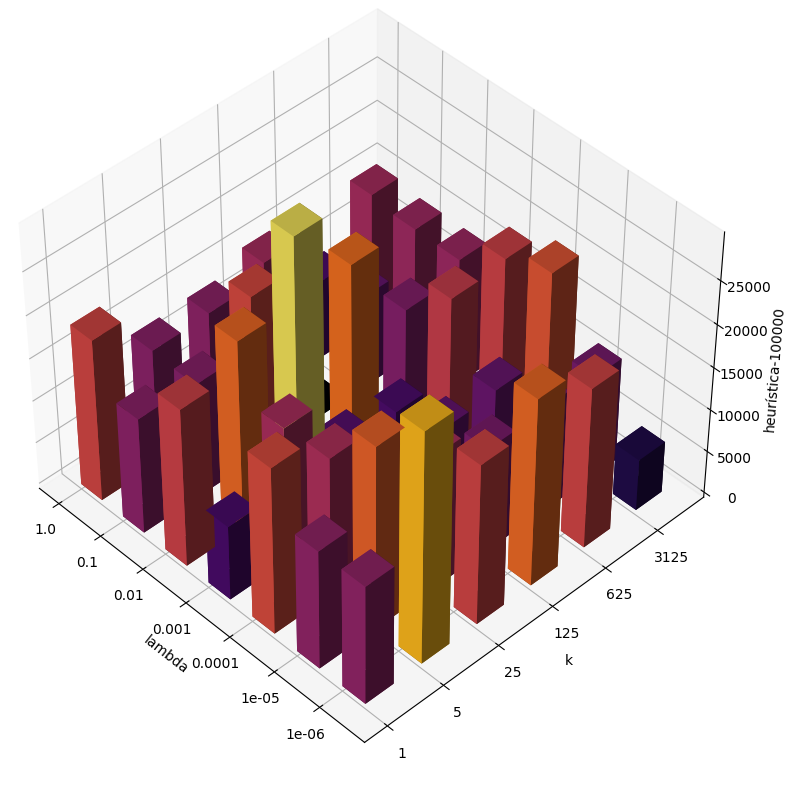
\includegraphics[scale=0.45]{images/experiment3.png}
\caption{Resultats de l'heurística per a $stiter=100$}
\centering
\end{figure}

\paragraph{Conclusions} Hem trobat que els valors màxims són donats per les variables $stiter=100$, $\lambda = 0.01$, i $k = 25$. Ens semblen nombres raonables tenint en compte el funcionament de l'algorisme simulated annealing, ja que no són valors massa extrems.

\newpage

\subsection{Experiment 4}
Aquest experiment ens planteja veure com evoluciona el temps d'execució en relació amb la magnitud del problema.
\paragraph{Observació} Si augmentem els paràmetres del problema, augmenta el temps d'execució.
\paragraph{Plantejament} Anem augmentant els paràmetres del problema fins a veure la tendència.
\paragraph{Hipòtesi} Creiem que l'algorisme Hill Climbing creixerà exponencialment en temps d'execució, donat que haurà de considerar moltíssims més successors possibles. Simulated Annealing, en canvi, no augmentarà molt el seu temps d'execució, però això repercutirà en una solució amb menor valor resultant que Hill Climbing pel fet que no realitzarà suficients passos per cobrir tot el problema.
\paragraph{Metodologia}
\begin{itemize}
\item Inicialment usarem els valors 10 centres de distribució i 100 gasolineres.
\item Usarem l'algorisme Hill Climbing i Simulated Annealing.
\item Executarem el programa amb llavor aleatòria i guardarem el temps d'execució per a cada algorisme (en aquest experiment no realitzem múltiples iteracions pel fet que el temps d'execució podria arribar a valors massa grans).
\item Augmentem els centres de distribució en 10 i les gasolineres en 100 i repetim.
\end{itemize}
\paragraph{Resultats} Hem obtingut els següents resultats:

\begin{figure}[htp]
\centering
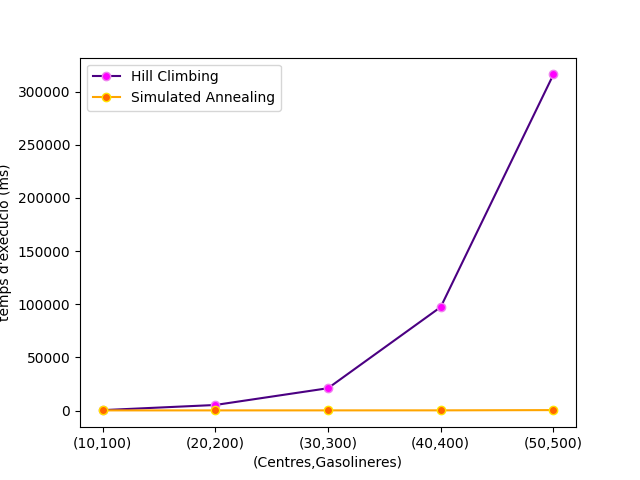
\includegraphics[scale=0.90]{images/experiment4.png}
\caption{Temps d'execució per a HC i SA}
\centering
\end{figure}

\begin{figure}[htp]
\centering
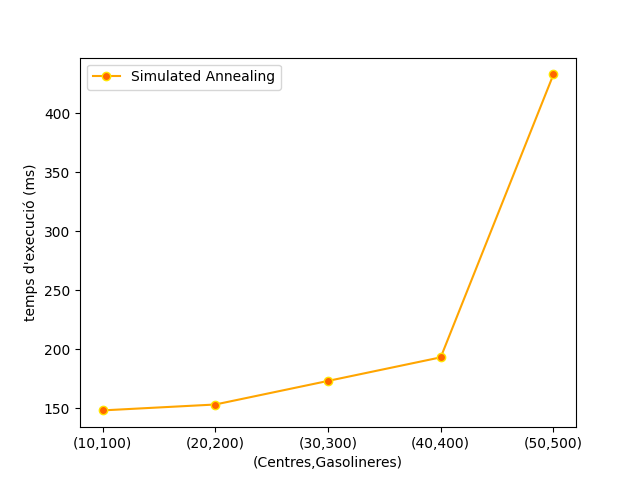
\includegraphics[scale=0.90]{images/experiment4-2.png}
\caption{Temps d'execució per a SA}
\centering
\end{figure}

Adicionalment, hem obtingut que per a 50 centres de distribució i 500 gasolineres l'algorisme Hill Climbing dona un valor de l'heurística de 618660,0, i Simulated Annealing una heurística de 617240,0.

\newpage
\paragraph{Conclusions} Podem veure com el temps d'execució d'ambdós algorismes augmenta quadràticament, però el cost de Hill Climbing augmenta molt més ràpid. Però contràriament a la nostra hipòtesi, podem veure com els resultats d'ambdós algorismes són comparables.\\

Els resultats d'aquest experiment podrien canviar si realitzéssim més iteracions per eliminar el paper de l'atzar i si seguissim probant magnituds del problema més grans (per exemple, potser HC acaba superant l'heurística de SA com hem hipotitzat). Però, els valors actuals ja triguen més de 5 minuts en computar-se i hem considerat inviable seguir.
\newpage

\subsection{Experiment 5}
Aquest experiment ens planteja augmentar el nombre de camions però reduir el nombre de centres de distribuició, i comparar el seu benefici i els quilòmetres recorreguts totals.
\paragraph{Observació} Reduir el nombre de centres, però mantenir el nombre de camions pot donar resultats diferents.
\paragraph{Plantejament} Executem el programa diverses vegades per cada escenari i comparem els resultats.
\paragraph{Hipòtesi} Si reduïm el nombre de centres de distribució es trobaran més dispersos i més distants a les gasolineres, per tant creiem que suposarà una reducció en els beneficis i un agument en la distància total recorreguda.
\paragraph{Metodologia}
\begin{itemize}
\item Usarem els valors 10 centres de distribució i 100 gasolineres
\item Usarem l'algorisme Hill Climbing.
\item Executarem el 100 vegades amb llavor aleatòria i guardarem els beneficis i els quilòmetres totals recorreguts.
\item Repetim el pas anterior amb 5 centres de distribució i 10 camions.
\end{itemize}
\paragraph{Resultats} Hem obtingut els següents resultats:

\begin{figure}[htp]
\centering
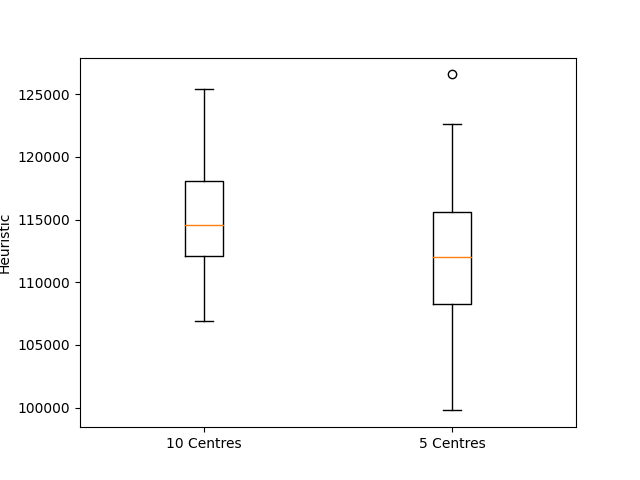
\includegraphics[scale=0.65]{images/experiment-5-2.png}
\caption{Valor de l'heurística per a ambdós escenaris}
\centering
\end{figure}

\begin{figure}[htp]
\centering
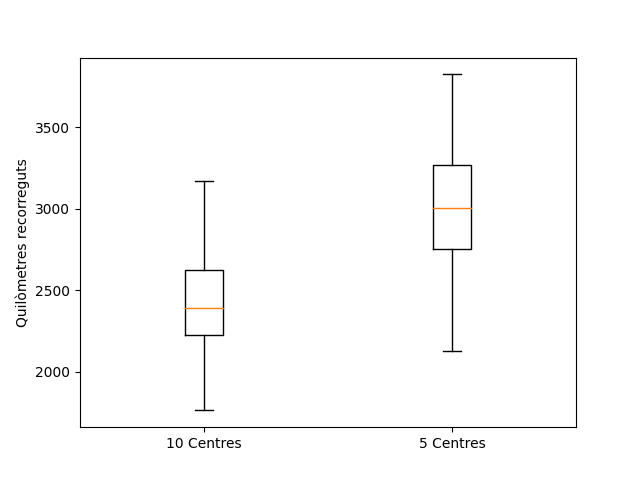
\includegraphics[scale=0.65]{images/experiment-5-1.png}
\caption{Quilòmetres totals recorreguts per a ambdós escenaris}
\centering
\end{figure}

\newpage
\paragraph{Conclusions} Com es pot veure, les nostres hipòtesis han resultat ser certes. Mantenir el nombre de camions, però reduir el nombre de centres de distribució suposa pitjors beneficis i més recorregut de mitjana.

\newpage

\subsection{Experiment 6}
Aquest experiment ens planteja anar augmentant el cost per quilòmetre i veure si això suposa un canvi en l'execució del problema, concretament en les peticions ateses segons els dies que duen pendents.
\paragraph{Observació} Augmentar el cost per quilòmetre podria alterar la resolució del problema.
\paragraph{Plantejament} Anem doblant el cost per quilòmetre i mesurant les peticions que són ateses.
\paragraph{Hipòtesi} Pensem que a mesura que anem augmentant el cost per quilòmetre les peticions més llunyanes tindran un cost per viatjar-hi superior al benefici que comportaria atendre-les, i per tant l'algorisme decidiria deixar-les sense atendre. Progressivament, a cada iteració hi haurà més peticions sense atendre, començant per aquelles amb menor benefici (i més dies pendents).
\paragraph{Metodologia}
\begin{itemize}
\item Usarem els valors 10 centres de distribució i 100 gasolineres
\item Usarem l'algorisme Hill Climbing.
\item Inicialment, establirem el preu per quilòmetre a 2.
\item Executarem el programa 200 vegades amb llavor aleatòria, i calculem el total de peticions ateses per a cada valor de dies pendents.
\item Dupliquem el preu per quilòmetre i repetim els passos anteriors fins a veure una tendència.
\end{itemize}

\paragraph{Resultats} Hem obtingut els següents resultats:

\begin{figure}[htp]
\centering
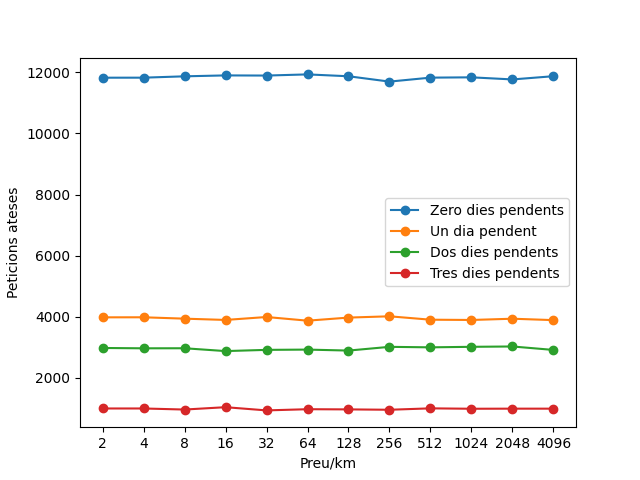
\includegraphics[scale=0.65]{images/experiment6.png}
\caption{Peticions ateses per Hill Climbing segons el preu per quilòmetre}
\centering
\end{figure}

Addicionalment, hem provat l'experiment amb un preu per quilòmetre arbitràriament gran i ens ha donat els mateixos resultats

\paragraph{Conclusions} Com es pot veure clarament, el preu per quilòmetre no influeix en les peticions ateses, contràriament a la nostra hipòtesi. Això és degut al tractament de les peticions inateses de la nostra heurística, que té en compte el viatge al centre més proper per calcular els seus beneficis. És a dir, si no paga el viatge avui l'haurà de pagar demà per menys benefici, així que les atén avui. Una heurística que tracti les peticions sense atendre diferent (per exemple, només mesurant les pèrdues respecte atendre-les avui) podria donar uns resultats diferents.

\newpage

\subsection{Experiment 7}
Aquest experiment ens planteja modificar el temps que treballa un camió en un dia, indirectament augmentant els quilòmetres màxims que podrà recórrer (sense modificar els 5 viatges diaris màxims).
\paragraph{Observació} Els quilòmetres màxims podrien limitar el nostre benefici.
\paragraph{Plantejament} Augmentem i reduïm la distància màxima i veiem la progressió.
\paragraph{Hipòtesi} A mesura que es va augmentant els quilòmetres màxims arribarà un punt on no suposarà cap millora, ja que ens limitaran els viatges màxims. Per tant, l'heurística pujarà fins a arribar a aquest punt, on es mantindrà estable per molt que pugin els quilòmetres màxims.
\paragraph{Metodologia}
\begin{itemize}
\item Usarem els valors 10 centres de distribució i 100 gasolineres.
\item Usarem l'algorisme Hill Climbing.
\item Executarem el programa 100 vegades amb llavors de generació aleatòria per a cada quantitat d'hores treballades entre 1 i 24 (addicionalment hem fet 15 minuts i 30 minuts).
\item Calculem la mitjana de cada valor,
\end{itemize}

\paragraph{Resultats} Hem obtingut els següents resultats:

\begin{figure}[htp]
\centering
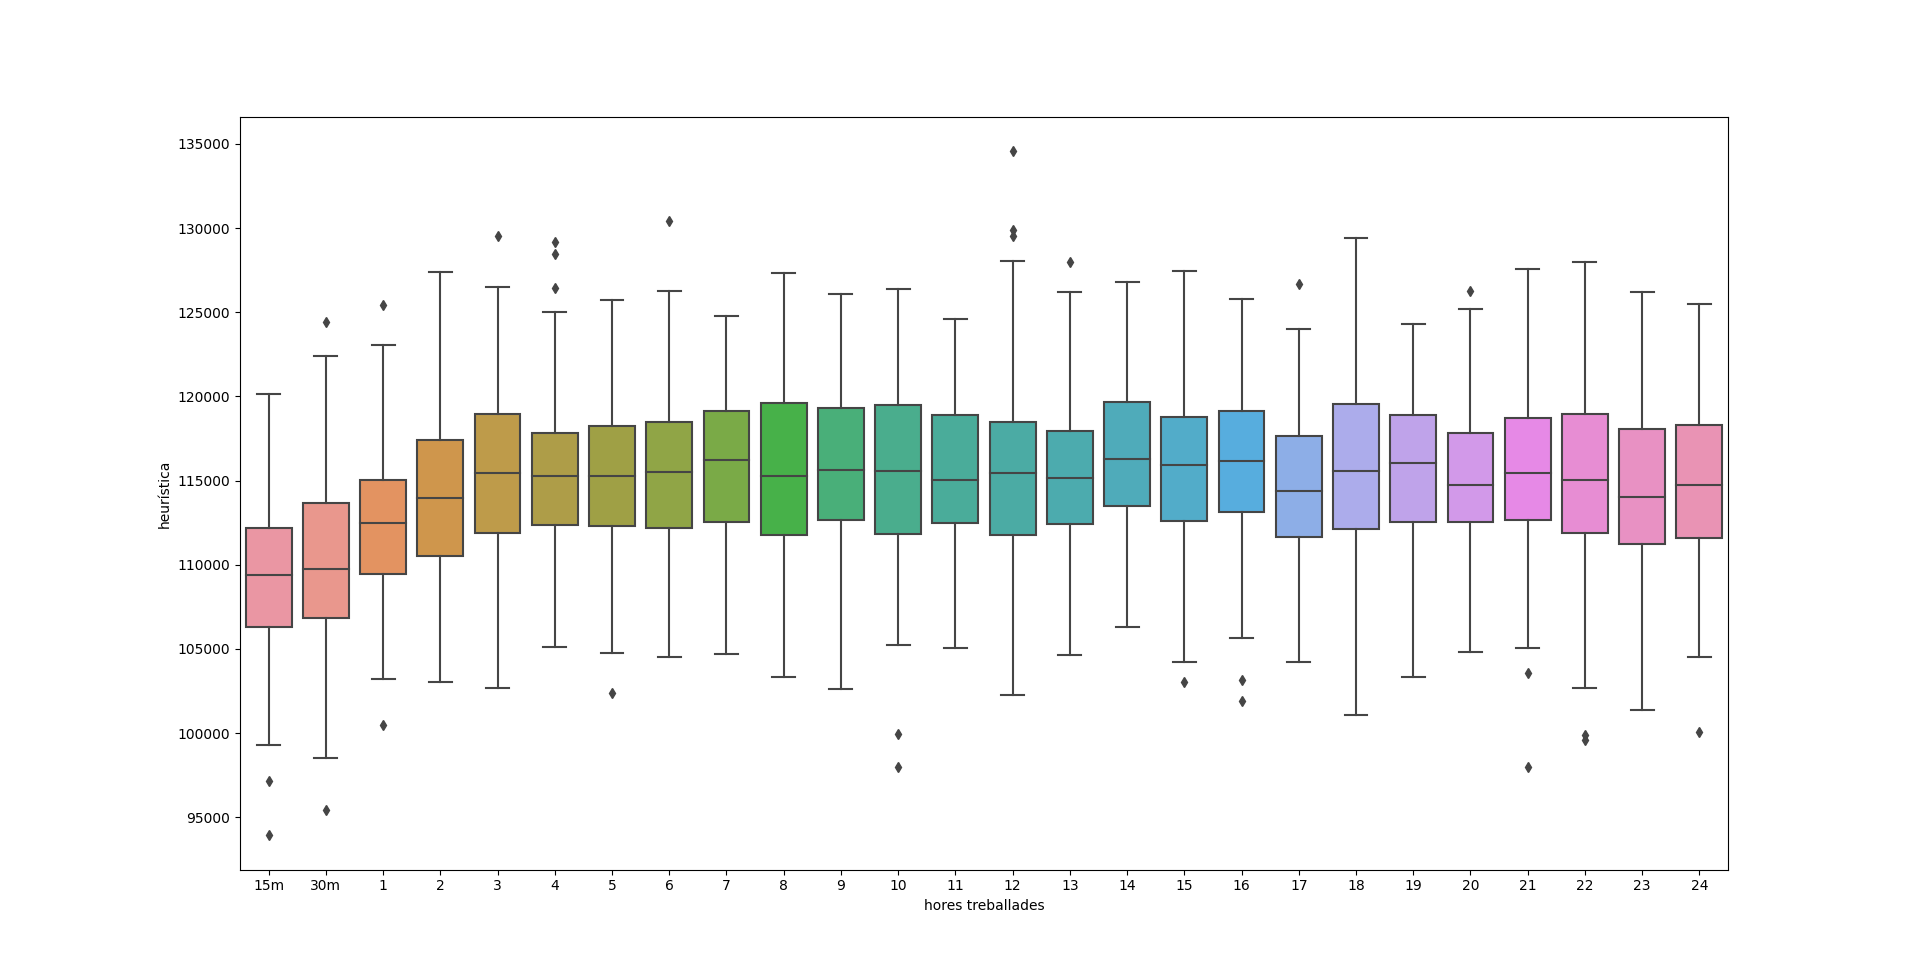
\includegraphics[scale=0.35]{images/experiment7-1.png}
\caption{Resultats segons el temps treballat entre 15 minuts i 24 hores}
\centering
\end{figure}

\begin{figure}[htp]
\centering
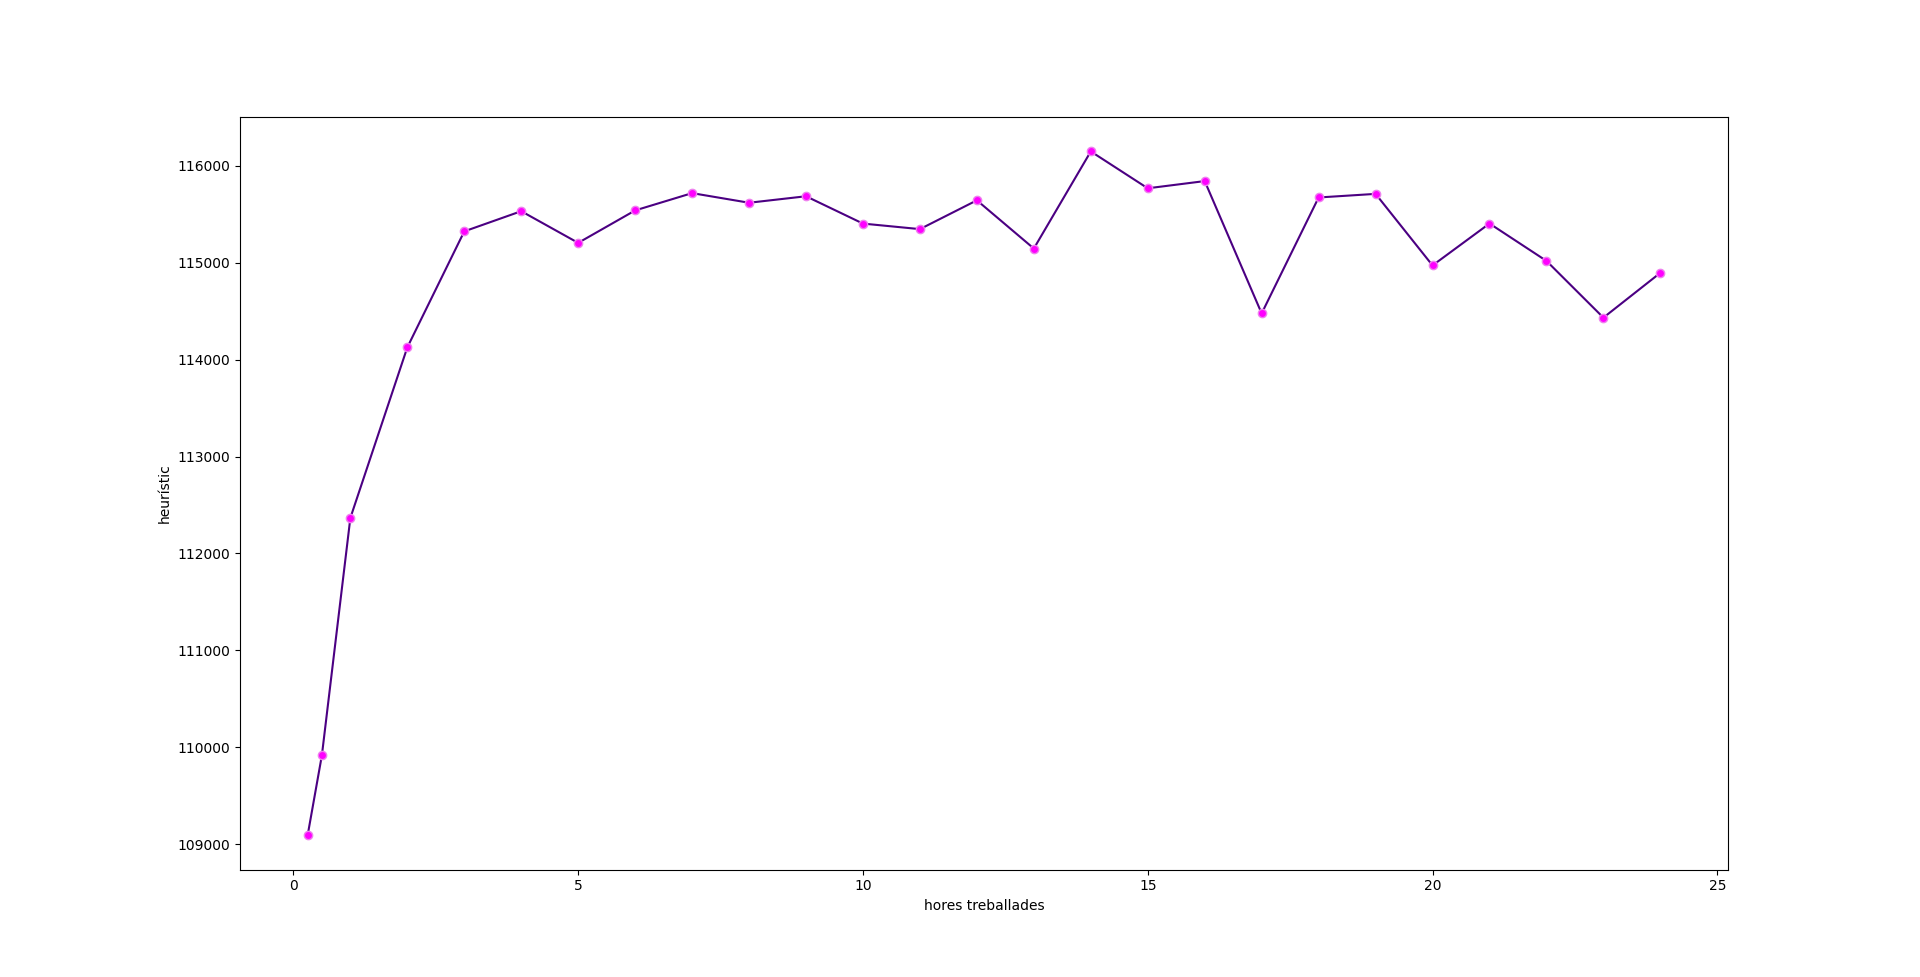
\includegraphics[scale=0.35]{images/experiment7-2.png}
\caption{Mitjana dels resultats segons el temps treballat entre 15 minuts i 24 hores}
\centering
\end{figure}

\newpage
\paragraph{Conclusions} Podem veure com la nostra hipòtesi era correcta, tot i que és sorprenent com arriba de ràpid a deixar de limitar els quilòmetres màxims, ja que passa entre només 2 i 3 hores. Les desigualtats passades aquest punt creiem que són el resultat de l'atzar, com es pot veure a la figura 21.

\newpage
\section{Conclusions}
Realitzar aquest treball ens ha donat una perspectiva molt més profunda sobre el funcionament dels algorismes Hill Climbing i Simulated Annealing, així com sobre els problemes de cerca local en general. Hem vist com són eines poderoses, donat que tinguis una representació adequada del problema i una bona funció heurística.\\

Hem comprovat com l'algorisme Simulated Annealing permet escapar màxims locals i obté solucions millors que Hill Climbing un cop hi calibres els paràmetres adequadament. També hem vist com, en problemes grans, SA obté solucions amb bondat comparable a HC en una fracció del temps.\\

Durant l'elaboració del treball hem tingut l'oportunitat de millorar els nostres coneixements sobre el programari Java, Python (concretament, la llibreria \emph{Matplotlib}), GitLab i \LaTeX, així com habilitats com el treball coordinat en equip i l'elaboració d'experiments per analitzar programari. Creiem que aquests coneixements els podrem aplicar durant la resta del grau i de la nostra carrera professional.\\

Finalment, creiem que el nostre grup ha tingut un bon funcionament intern i estem orgullosos del resultat final, tant en programació com en documentació, i esperem seguir treballant junts en altres treballs de l'assignatura.

\newpage
\section{Treball d'Innovació: DLSS}
\subsection{Tema Seleccionat}
\emph{NVIDIA Corporation} ha desenvolupat en els últims anys un parell d'eines que suposen la introducció de la IA al món dels gràfics en temps real per a l'usuari comú. Aquestes són la seva tecnologia de Raytracing$^{[2]}$, i DLSS$^{[1]}$, que vol dir \emph{Deep Learning Super Sampling}. Mentre que Raytracing s'ha estat emportant gran part dels mèrits i atenció, nosaltres creiem que DLSS té un impacte molt major en l'usuari comú. Aquesta nova tecnologia permet que amb una quantitat de recursos molt menor, i en conseqüència amb un impacte econòmic i ecològic menys significatiu, es puguin obtenir els resultats que prèviament requerien l'ús de targetes gràfiques significativament més avançades. Això, addicionalment, també permetrà allargar la vida útil d'aquest hardware.

\subsection{Responsabilitats de l'equip}
Hem repartit les tasques de la següent manera:

\paragraph{Pol Marcet Sardà:} Desenvolupament d'un exemple de prova, ja sigui a través de la SDK pública proporcionada per Nvidia$^{[3]}$, o a través d'un dels connectors per als motors gràfics més utilitzats, Unity$^{[4]}$, o Unreal Engine$^{[5]}$. Si es procedeix adequadament en el desenvolupament de l'exemple de l'SDK, també s'intentarà realitzar la integració de la SDK amb un motor real en desenvolupament privatiu, que Pol Marcet Sardà està desenvolupant. Es llicenciarà una còpia del codi font de la llibreria gràfica per a la universitat per tal que aquesta pugui avaluar el codi, així com una llicència per a una còpia de l'executable compilat de tot el motor per a la seva demostració.

\paragraph{Adria Fernandez Clemente:} Realitzarà un estudi estadístic i comparatiu entre el rendiment i qualitat de diferents títols amb aquesta capacitat per a veure l'impacte que aquesta tecnologia té. Actualment, la llista de títols on es realitzaran les proves són: Cyberpunk 2077, Doom Eternal i No Man's Sky, tot i que la llista de títols pot variar.

\paragraph{Pablo Vega Gallego:} Investigació del funcionament intern de la IA aplicada per NVIDIA. Desafortunadament, NVIDIA no proporciona detalls tècnics sobre la implementació més enllà del fet que fan ús dels nous tensor cores$^{[6]}$ de la seva nova línia de productes, que s'explicarà en tant detall com sigui disponible. També s'explicarà com funcionen les IA d'upscaling a través de \emph{combolutional neural networks}$^{[7]}$, ja que és l'aproximació més probable realitzada per NVIDIA.

\subsection{Dificultats}
A causa de la manca d'informació proporcionada per NVIDIA sobre els detalls més específics d'implementació, hi ha un cert nivell d'especulació a l'hora d'explicar com funciona a escala conceptual. Afortunadament, aquest és un camp amb estudis detallats al respecte, i creiem que podem donar una explicació vàlida i prou acurada a la realitat.\\

Actualment tenim a la nostra disposició una targeta RTX 2080, una targeta RTX 3060, una targeta RTX 3070 i una targeta RTX 970, i creiem que ens donen un ventall ampli de capacitats que seran útils per a l'experimentació.

\newpage

\subsection{Progrés Realitzat}
S'han fet unes proves preliminars amb la SDK de NVIDIA i el codi d'exemple proporcionat, compilat amb VS 2019. Queda investigar si es pot compilar amb GCC o Clang en compatibilitat Mingw-w64. A continuació pot trobar una captura del programa realitzat. Encara no s'ha estructurat un projecte d'entrega.

\begin{figure}[htp]
\centering
\includegraphics[scale=0.35]{images/TrebInnovTest.jpg}
\caption{Projecte proporcionat per NVIDIA corrent sobre la RTX 2080)}
\centering
\end{figure}

\subsection{Fonts}

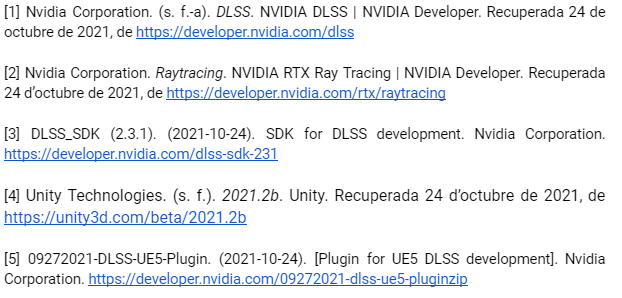
\includegraphics[scale=0.95]{images/fonts.PNG}

\end{document}